
% Literature Review 

% Talk about standard RNNs, pre-transformers era? Why was there no NAT in this era? 

% Brief intro about transformers? Why is it so ubiquitous in today’s research 

% Problems in NAT 

% Removal of Autoregressive factorization across time 

% Multimodality problem 

% Where has NA-solution been done before? 

% Solutions 

% Iterative Refinement 

% Semi-autoregressive - Trade off between faster generation and quality 

% Distilled training data – reduce number of modes 

% Limitations of this solutions – iterative refinement requires complex solutions and architectures. 

This chapter aims to provide a comprehensive literature review of research done for non-autoregressive transformer models. This section will first briefly cover methods for sequence to sequence prior to the era of the transformer \cite{vaswani_attention_2017}; for which the need for non-autoregressive methods was not so pressing. After which, we will provide a summary of the transformer architecture \cite{vaswani_attention_2017} and then examine different non-autoregressive methods.

It is important to note that non-autoregressive methods are not completely new and unheard of. There has been methods and algorithms proposed in other domains. We will dedicate the last section of this chapter to those methods. 



\section{Background and History} \label{sec:background}
\subsection{Autoregressive Methods for sequence to sequence generation} \label{subsec:background1}
Prior to the advent of transformers models in 2017 \cite{vaswani_attention_2017}, the defacto models to use for sequence to sequence generation were variants of Recurrent Neural Network \cite{elman_distributed_1991}, such as the Long Short Term Memory \cite{lstm_original}, Gated Recurrent Unit \cite{gru_paper}. At inference time, these models generate words via an autoregressive factorization, following the equation:

\begin{equation} \label{eqn:autoregressive_factorization} P(y|x) = \prod_{t=1}^{T}p(y_t|y_{<T},x) \end{equation}

This autoregressive factorization assumes casual conditional dependence between the current decoding step and the output of the previous decoding step, thus generating the sequence from left to right. This implementation also permits the training of the models to be relatively straightforward by simply minimizing the negative log likelihood of Equation \ref{eqn:autoregressive_factorization}, allowing for training methods as teacher forcing \cite{williams_learning_1989_teacher_forcing}.

The need for non-autoregressive methods were not as vital then, as the autoregressive factorization were thought to be one of the advantages of RNNs variants in order to induce temporal invariance \cite{battaglia_relational_inductive_biases_2018} in the model. The size of RNN models were also relatively smaller compared to today. The need for non-autoregressive methods stemmed from the increased popularity in model variants of the transformer \cite{vaswani_attention_2017}. In the next subsection, we will concisely cover the transformer architecture, and explain the demand for non-autoregressive methods.


\subsection{Transformer}\label{subsec:background2}
\textcite{vaswani_attention_2017} proposed the transformer in 2017. Since then, many model variants have been introduced to take advantage of its exceptional language modeling capabilities, At the core of the transformer architecture is an unique self-attention mechanism used to model dependencies independent of their respective positions in the input or output sequence \cite{vaswani_attention_2017}.The transformer follows an encoder-decoder structure \cite{cho_learning_2014_encdec, sutskever_sequence_2014_encdec, bahdanau_neural_2016_encdec} consisting of stacks of self-attention, feed-forward, and layer normalization.This formulation allows the transformer to scale up to huge sizes on huge training data by leveraging on hardware and the ability to be parallelized during the training process. 
% should i go into more specific detail about transformer?


Since then, many different transformer variants \cite{wolf-etal-2020-transformers} have been proposed for a multitude of purposes. For instance, BERT \cite{devlin_bert_2019} gave rise to the trend of using contextualized word embeddings, which soon proved to be superior to static word embeddings such as word2vec \cite{mikolov_efficient_2013_word2vec}. As a consequence, transfer learning became a popular method to adapt the publicly available pretrained BERT model for fine-tuning on downstream tasks such as word sense disambiguation \cite{yap_adapting_2020}. Transformers have also been applied to sequence to sequence tasks. Notable models include GPT-2 \cite{radford_language_nodate_gpt2}, GPT-3 \cite{brown_language_2020_gpt3}, both of which was trained on a huge corpus of text data and has since surpassed many benchmarks and shown potential for few-shot learning for many tasks such as story generation and even simple arithmetic.

\subsubsection{An example of Transfer Learning}\label{subsubsec:transfer_learning_me}

\label{subsec:transfer_learning}
\begin{figure}[hpbt!]
    \centering
    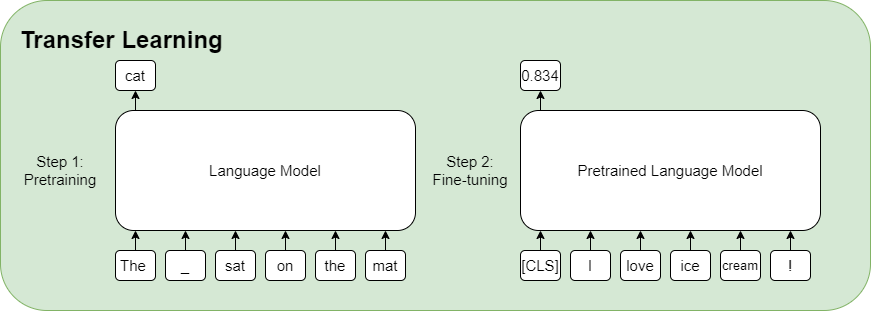
\includegraphics[scale=0.5]{images/chap02_images/transfer_learning_toy_example.png}
    \caption{An straightforward example of how transfer learning is usually done. A language model is pretrained first using a language modeling task. These pretrained language models are availably readily online. Thereafter, the pretrained language model is finetuned on a downstream task. In this example, it is trained on sentiment analysis and is used to output a sentiment score.}
    \label{fig:transfer_learning_toy_example}
\end{figure}
Transfer learning \cite{zhuang_comprehensive_2020_transfer_learning} is a common machine learning technique which aims to adapt the information in a trained model to a related domain. In today's Natural Language Processing landscape, transfer learning is made ubiquitous and popular by the ease of access of pretrained language models like BERT \cite{devlin_bert_2019}. Using transfer learning (Toy example in Figure \ref{fig:transfer_learning_toy_example}) allows us to use pretrained models and possibly save lots of compute time.

\textcite{yap_adapting_2020} used transfer learning to adapt a BERT \cite{devlin_bert_2019} pretrained model to a word sense disambiguation task. Pretraining is done by training BERT trained on gigabytes of text data on a masked language modeling task, allowing it to learn contextualized word representations. The pretrained BERT is publicly available at many open source repositories. \textcite{yap_adapting_2020} then fine-tuned the pretrained BERT model on the gloss selection task. In doing so, the gloss selection task allowed the BERT model to break state of the art on the word sense disambiguation task. 

Transfer learning is a tried and tested method to adapt models across different domains. In this work, we will also utilize transfer learning. Section \ref{subsec:transfer_learning} covers this usage in details.

\subsection{Drawbacks of the transformer} \label{subsec:drawbacks_transformer}

\subsubsection{Loss of inductive bias} \label{subsubsec:drawback1_inductive_bias}
Unlike the recurrent neural network whose recurrent structure induces temporal invariance and locality bias in the model \cite{battaglia_relational_inductive_biases_2018}, the feed-forward layers and self-attention layer in the transformer does not has any relational inductive bias \cite{battaglia_relational_inductive_biases_2018}. In other words, the transformer sacrifices the temporal invariance for greater modeling capacity and scaling potential. 

\subsubsection{Steady increase of model size over the years} \label{subsubsec:drawback2_increasing model size}

%todo plot model sizes?
The ease of scaling of transformers to hundreds of gigabytes in data has also led models sizes to steadily increase. The original transformer \cite{vaswani_attention_2017} had only 66 million parameters. BERT, in 2018, \cite{devlin_bert_2019} had 110 million parameters. By 2020, Turing-NLG had 17 billion\footnote{https://www.microsoft.com/en-us/research/blog/turing-nlg-a-17-billion-parameter-language-model-by-microsoft/} \cite{ganesh2020compressing_turingNLG_param_ref}, and GPT-3 \cite{brown_language_2020_gpt3} had an even larger 175 billion, dwarfing its predecessors significantly in size. Recently in 2021, Microsoft released the Switch Transformer \cite{fedus2021switch}, which has a gigantic trillion parameters.

This trend has raised questions in the research community about the practicality and impact \cite{schwartz_green_ai_2019} of large models. These large models are expensive to run and a large amount of computational power and memory is required just for a single forward pass through the model. As a result, there has been work looking to compress these large models, either via knowledge distillation \cite{hinton_distilling_2015} to train a smaller model \cite{sanh_distilbert_2020}, or by pruning \cite{rogers_primer_in_bert_2020,chen_lottery_2020,frankle_lottery_2019} models to reduce computation.

In a similar vein, non-autoregressive transformer models aim to speed up generation by generating more or all tokens in a single forward pass of the model. This allows for huge savings in computational power compared to  autoregressive transformer sequence to sequence models \cite{vaswani_attention_2017, brown_language_2020_gpt3, radford_language_nodate_gpt2} which can only generative one token per forward pass.



\section{Non-autoregressive Transformer sequence to sequence Models} \label{sec:NAT model}

\subsection{Problem Definition} \label{subsec:problem_def}
Non-autoregressive sequence generation aims to speed up decoding by removing the autoregressive factorization in Equation \ref{eqn:autoregressive_factorization}. At its most simplest and naive form, non-autoregressive generation can be formulated as:

\begin{equation}
\label{eqn:naive_non_autoregressive_formulation} 
P(Y|X) = \cdot \prod_{t=1}^{T}p(y_t|x_{1:T^\prime})
\end{equation}

where generation is only dependent on the very first input sequence. This formulation is straightforward, and training can be done similarly to autoregressive training by minimizing the negative log-likelihood.

However, the removal of conditional dependence across time has created several problems at the cost of faster generation. In the next subsection, we will explain these problems.

\subsection{Obstacles to realizing a deployable non-autoregressive sequence to sequence model} 
\label{subsec:obstacles_NAT}
In this section, we will examine different problems arising from the lack of the autoregressive factorization in non-autoregressive sequence generation.
\subsubsection{Length Prediction} \label{subsubsec:nat_prob_length}
As mentioned in Section \ref{sec:background}, autoregressive sequence generation decodes the sequence token by token. The decoding algorithm stops when the end of sequence token is generated in the latest decoding step. This heuristic is uncomplicated and works well practically. On the other hand, non-autoregressive sequence generation is not afforded this advantage as either any part or the whole of the sequence is generated in one decoding step. Therefore, there is a need to predict or assume the length of the output sequence in non-autoregressive sequence generation. 

\textcite{gu_non-autoregressive_2018} circumvents this by naively modelling the output sequence length using a separate conditional distribution $P_L$. Thus, Equation \ref{eqn:naive_non_autoregressive_formulation} becomes:
\begin{equation}
\label{eqn:gu_non_autoregressive_formulation} 
P(Y|X;\theta) = p_L(T|x_{1:T^\prime};\theta) \cdot \prod_{t=1}^{T}p(y_t|x_{1:T^\prime};\theta)
\end{equation}

Several authors choose to espouse this approach of modeling the length of the output sequence, either by dynamically changing the output sequence length with each decoding step using a length heuristic or prediction module \cite{gu_levenshtein_2019,chan_kermit_2019,chan_multilingual_kermit,ran_learning_to_recover_2020,stern_insertion_2019,zhou_improving_2020_with_monolingual_data, ran_guiding_2020_reordering,ma_flowseq_2019}, or by predicting a static output sequence length \cite{gu_non-autoregressive_2018,zhou_improving_2020_with_monolingual_data,ghazvininejad_mask-predict_2019, qian_glancing_2020}. Other methods assume a fixed sequence length during decoding \cite{wang_semi-autoregressive_2018,guo_non-autoregressive_2020_image_captioning,saharia_non-autoregressive_2020_latent_alignment,chan_imputer_2020,bao_non-autoregressive_2019_position_learning, guo_fine-tuning_2019_curriculum,ding_context-aware_2020} at the cost of flexibility of the generated sequence and a potential issue of choosing the wrong sequence length.

\subsubsection{Multi-modality Problem} \label{subsubsec:nat_prob_multimodal}
An arguably bigger problem to non-autoregressive sequence generation is its strong decline in generation quality. Autoregressive sequence generation implicitly models the strong casual correlation across time \cite{gu_non-autoregressive_2018} when decoding. Removing the autoregressive factorization causes the model to lose that ability. As a result, the multi-modality problem arises \cite{gu_non-autoregressive_2018, zhou_understanding_2020}. This problem often manifests itself in sequence generation as token repetition \cite{ran_learning_to_recover_2020}.

\begin{figure}[hpbt!]

    \centering
    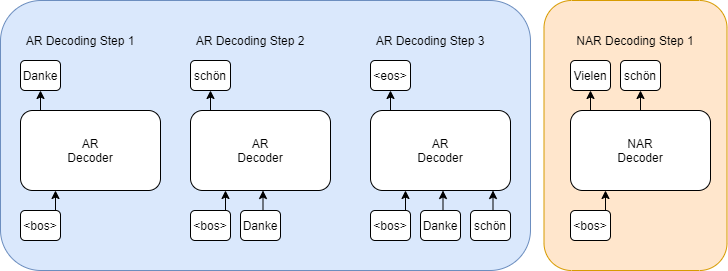
\includegraphics[width=\textwidth]{images/chap02_images/AT_vs_NAT.png}
    \caption{Comparison of the decoding process in an autoregressive model (left) and a non-autoregressive model (right). The non-autoregressive model is able to generate the next token based on the sequence generated in the previous step, while the non-autoregressive model does not do so and hence assumes conditional independence between each output token.}
    \label{fig:AT_vs_NAT}
\end{figure}

\begin{figure}[hpbt!]

    \centering
    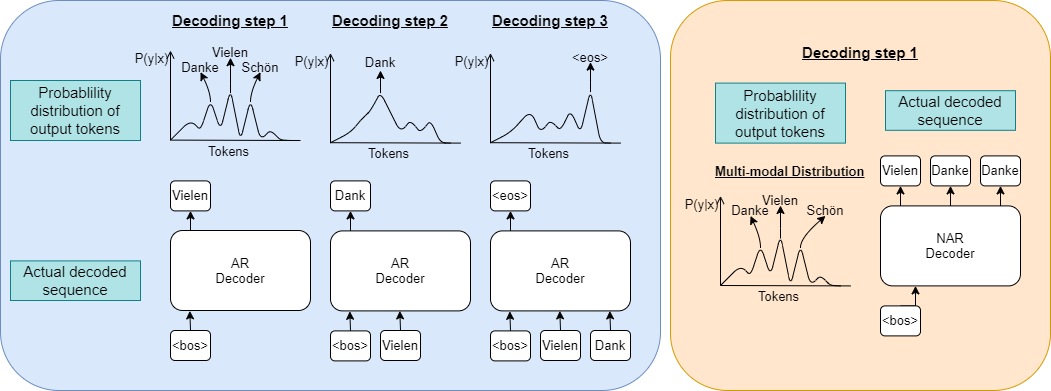
\includegraphics[width=\textwidth]{images/chap02_images/AT_vs_NAT_distributions.png}
    \caption{A simplified view of how the multimodality problem manifests in non-autoregressive sequence generation. 'Danke', 'Vielen', 'schön' are the multiple modes of the  initial probability distribution. \textbf{Left:} Autoregressive sequence generation decodes a single mode from the multiple available modes. In subsequent decoding steps, the number of modes in the distribution is reduced. \textbf{Right:} Non-autoregressive sequence generation typically has to choose multiple tokens from multiple modes, and therefore leads to repetitive tokens in its generation.}
    \label{fig:AT_vs_NAT_distribution}
\end{figure}
% not working
% \begin{figure}[htbp]
%   \centering
%   \includesvg{images/chap02_images/AT_vs_NAT.svg}
%   \caption{svg image}
% \end{figure}


The multi-modality problem is defined by \textcite{gu_non-autoregressive_2018} as the inability to accurately reflect the conditional independence of each word in the sequence using a single target distribution. For example \cite{gu_non-autoregressive_2018}, the English phrase 'Thank you' can be translated correctly into `Danke', `Danke schön', or `Vielen Dank' in German. As an non-autoregressive model would most likely generate the whole sequence in one decoding step, it is possible that `Danke Dank' or `Vielen schön' gets produced. This is because there is no conditional dependence between the first word and the second word. In other words, the generation of the second word does not rely on the first word. This is depicted in Figure \ref{fig:AT_vs_NAT}. 

`Danke', `Vielen', `schön' are all highly possible outputs of the model, and hence are referred to as `modes'. At decoding time, the non-autoregressive model is not prohibited from choosing conflicting modes to use in the output sequence, nor is it able to determine if a mode has already been or will be chosen for another position. Figure \ref{fig:AT_vs_NAT_distribution} further illustrates this phenomenon. Therefore, the problem of decoding conflicting modes is referred to as the multi-modality problem.

\section{Solutions and Approaches} \label{sec:solutions}

In this section, we will discuss the different approaches towards the problems metioned in Section \ref{subsec:obstacles_NAT}. Many of these approaches are used in conjuction with the other approaches mentioned below.
% Iterative Refinement 
% Semi-autoregressive - Trade off between faster generation and quality 
% Distilled training data – reduce number of modes 
% Fertilities  
% Limitations of these solutions – iterative refinement requires complex solutions and architectures. 

\subsection{Sequence Level Knowledge Distillation}
\label{subsec:sol1_slkd}
%put  image on example of how slkd is done here
\begin{figure}[h!]
    \centering
    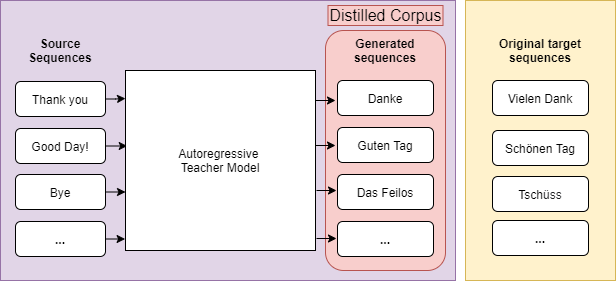
\includegraphics[width=\textwidth]{images/chap02_images/seq_level_kd.png}
    \caption{Sequence level knowledge distillation. The original training data is fed through an autoregressive teacher model first. The distilled corpus is formed by collecting all the generated outputs paired with the same original source sequence.}
    \label{fig:slkd}
\end{figure}


Knowledge Distillation is the most common approach used to tackle the multi-modality problem mentioned in Section \ref{subsubsec:nat_prob_multimodal}. With the exception of \cite{ran_learning_to_recover_2020}, almost all work in non-autoregressive research \cite{ren_study_2020_comma, gu_non-autoregressive_2018, gu_levenshtein_2019, guo_non-autoregressive_2020_image_captioning, bao_non-autoregressive_2019_position_learning, wang_semi-autoregressive_2018,saharia_non-autoregressive_2020_latent_alignment, chan_kermit_2019, chan_multilingual_kermit, ghazvininejad_mask-predict_2019,stern_insertion_2019, zhou_improving_2020_with_monolingual_data, ran_guiding_2020_reordering, ma_flowseq_2019, qian_glancing_2020, guo_fine-tuning_2019_curriculum, ding_context-aware_2020} use sequence level knowledge distillation \cite{kim_sequence-level_2016_knowledge_distillation} for training in the domain of machine translation. Sequence level knowledge distillation is done by first training a teacher autoregressive model, and then passing the source training data through the autoregressive model to get the predicted sequence from the model. These generated outputs are paired with the same source sequences and used as distilled training data for the non-autoregressive model. This process is shown in Figure \ref{fig:slkd}.

\textcite{zhou_understanding_2020} quantified the effectiveness of sequence level knowledge distillation in his work. They found empirical evidence that the use of the autoregressive model to generate a new set of training data significantly reduced the number of modes in the new training data. Specifically, \textcite{zhou_understanding_2020} used a measure of complexity and faithfulness to the original training data. They found that models with low capacity such as the vanilla non-autoregressive model \cite{gu_non-autoregressive_2018} prefered training data with lower complexity, while models with higher capacity such as the Levenstein Transformer \cite{gu_levenshtein_2019} preferred training data with higher complexity. Using distilled data greatly mitigates the multi-modality problem mentioned in Section \ref{subsubsec:nat_prob_multimodal}, thereby boosting the quality of the generated sentence.

\subsection{Fertilities} \label{subsec:sol2_fertilities}
\textcite{gu_non-autoregressive_2018} first introduced the vanilla non-autoregressive transformer which aims to tackle the multimodality problem using fertilities. Fertilities determine the number of words in the target sentence that each word in the source sentence corresponds to. Therefore, the length of the target sequence can be easily calculated by summing the fertilities, while at the same time providing the model with an intermediate factorization of the output space. \textcite{gu_non-autoregressive_2018} modeled the fertilities $p_F(f_{t^\prime}|x_{1:T^\prime})$ using a simple feedforward linear layer with a softmax classifier at output encoder embedding of each input token. The casual mask of the decoder was also removed so that the whole sequence could be generated simultaneously. 

However, this approach was criticized as limited in terms of expressiveness \cite{ma_flowseq_2019} and was unable to properly model the interdependence between words in the output sequence. Subsequent work mostly focused on other approaches and used variants of iterative refinement algorithms. 

\subsection{Iterative Generation} \label{subsec:sol3_iterative_generation}
Due to the limited modeling capacity of fertilities, not many research work espoused this approach. Instead, many authors chose to deal with a tradeoff between the number of decoding steps and generation quality via the iterative refinement approach. Typically, the more the number of decoding steps, the higher the quality of the sequence. There are several methods along this approach. Most work chose to increase the number of decoding steps in order to improve the generation quality. It is hypothesized \cite{ghazvininejad_mask-predict_2019} that iterative sequence generation helps to collapse the modes in the distribution, thus alleviating the multi-modality problem. There are two main approaches, left-to-right non-autoregressive sequence generation, and arbitary-position non-autoregressive sequence generation. This is depicted in Figure \ref{fig:leftright_vs_arbitrary}.


\begin{figure}[hbtp!]
    \centering
    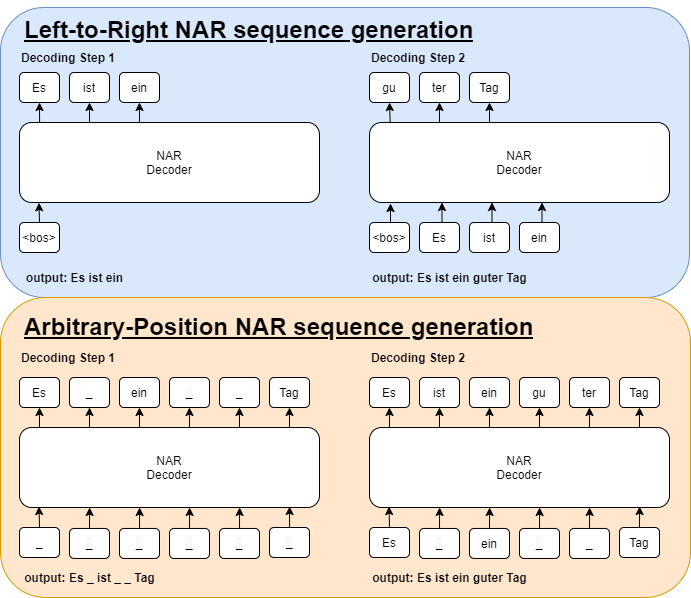
\includegraphics[width=\textwidth]{images/chap02_images/leftright_vs_arbitrary.png}
    \caption{Visualization of a simplified decoding process of the two non-autoregressive sequence generation approaches. \textbf{Top:} Left to right non-autoregressive sequence generation. It resembles the left-to-right autoregressive sequence generaiton, except that more than one token is predicted with decoding step. \textbf{Bottom:} Arbitrary-Position NAR sequence generation. A blank canvass is fed to the decoder and the decoder fills in the canvass at any possible. Note that this is simplified, most models use a more complicated heuristic.}
    \label{fig:leftright_vs_arbitrary}
\end{figure}
%put image of left-right vs arbitary position here


\subsubsection{Left-to-right non-autoregressive Sequence Generation} \label{subsubsec:sol3_iterative_generation_left2right}
This method resembles left-to-right autoregressive sequence generation, except that groups of tokens are generated with every decoding step. This approach is not common.

Currently, only the Semi-Autoregressive Transformer \cite{wang_semi-autoregressive_2018} espouses this approach. The Semi-Autoregressive Transformer uses a relaxed causal attention mask along with a group level chain rule to predict the next group of tokens. Using different forms of attention masks, the Semi-Autoregressive Transformer performs long and short distance prediction of tokens. In this work, we also use left-to-right non-autoregressive sequence generation.

\subsubsection{Arbitary-position non-autoregressive sequence generation} \label{subsubsec:sol3_iterative_generation_arbirtary_position}
Models in this section generate tokens on a canvas. The generated tokens can be placed anywhere in the sequence; it does not have to be from left to right. The positions of the generated tokens are decided either via a heuristic or a classification task depending on the setup of the model. 

These are some examples of models espousing this approach. The Levenshtein Transformer \cite{gu_levenshtein_2019} takes inspiration from the Levenshtein distance \cite{Levenshtein1965BinaryCC_lev_distance} and iteratively suggests token insertion and deletion operations on a canvas. KERMIT \cite{chan_kermit_2019, chan_multilingual_kermit} and the Insertion Transformer \cite{stern_insertion_2019} also takes a similar insertion-only approach by placing predicted tokens in between slots in a sequence.  Similarly, the Imputer \cite{chan_imputer_2020},a latent alignment model, assumes a monotonic mapping between token alignment predictions and the target sequence in order to fill in a canvas. These models work relatively well, however, they are complex to train and use.

% lev trans, semi-auto, latent alignment, imputer, kermit, multi-kermit, insertion, 

\subsection{Supplementing generation with external knowledge} \label{subsec:sol4_external_knowledge}
% position learning, reorder, monolingual, flowseq,
The methods in this section incorporates external knowledge via latent variables into the encoder or decoder of the transformer to improve non-autoregressive sequence generation. Unless mentioned otherwise, all models in this section follow that of the vanilla non-autoregressive transformer \cite{gu_non-autoregressive_2018}; the whole sequence is generated in one decoding step. 

PNAT \cite{bao_non-autoregressive_2019_position_learning} creates a position predictor module for the model to model the positions of the sequences. The module produces a latent variable which is then incorporated into the decoder input.

In another vein, \textcite{zhou_improving_2020_with_monolingual_data} supplements the non-autoregressive transformer by adding more data from a monolingual dataset of the source language. The additional dataset is fed through a separate trained autoregressive model to produce the sequences in the target language. The additional data is then used in conjuction with the original parallel dataset to train the model.

Unlike all the other approaches, Flowseq \cite{ma_flowseq_2019} further reinvents the wheel by using flow based generative models \cite{rezende_variational_2016_flow} instead of the transformer. Using a chain of invertible operations, a simple distribution is modelled into a complex distribution \cite{ma_flowseq_2019}. The use of generative flow also allows the use of Recurrent Neural Networks, while still keeping the non-autoregressive property. 


\subsection{Post-Editing} \label{subsec:sol5_post_editing}
Post-editing, also commonly known as sequence refinement, is a relatively recent technique applied to non-autoregressive generation. It refers to modifying or improving the sequence that has been already generated. This can be done in the next decoding step as part of the generation process.

As mentioned in Section \ref{subsubsec:sol3_iterative_generation_arbirtary_position}, \textcite{gu_levenshtein_2019} applies post editing as part of its Levenshtein Transformer. It uses a token deletion operation to dynamically delete tokens that are deemed to be incorrect, and the token insertion operation can add to the sequence. 
Mask-Predict \cite{ghazvininejad_mask-predict_2019} generates the whole sequence in one decoding step, but indicates uncertainty in its generation by masking some tokens out. In the next decoding step, the model re-predicts the masked tokens. RecoverSAT \cite{ran_learning_to_recover_2020} also generates segments of tokens simulateously, then removing repetitive segments indicated by a deletion token. Lastly, the Glancing Transformer \cite{qian_glancing_2020} adopts a 3 stage decoding process. First, the model decodes the whole sequence. Then, it conducts a novel glancing operation to determine which words are likely to be wrong. Finally, the models samples from the probability distribution to update the sequence.
% lev trans, mask predict, learning to recover,
